\section{Биматрична игра по варианту}

Рассмотрим биматричную игру 2x2, заданную по варианту. Вывод программы представлен на
рисунке~\ref{fig:fig05}.

\begin{figure}
  \centering
  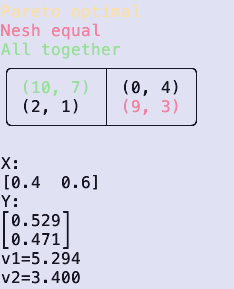
\includegraphics[scale=0.7]{../../artifacts/lw3/variant_game.png}
  \caption{Биматричная игра по варианту 2x2}
  \label{fig:fig05}
\end{figure}

Как видим, у этой игры есть две равновесные по Нешу систуации в чистых стратегиях,
поэтому в смешанном дополнении игры существует еще одна вполне смешанная ситуация
равновесия, которую мы можем рассчитать по формулам из теоремы~\ref{th1}.

\begin{theorem}\label{th1}
Пусть $\Gamma(A,B)$ --- биматричная (2$\times$2)-игра, где $A$ и $B$ 
являются невырожденными матрицами:
\[
(A, B) \;=\;
\begin{pmatrix}
(\alpha_1, \beta_1) & (\alpha_1, \beta_2)\\
(\alpha_2, \beta_1) & (\alpha_2, \beta_2)
\end{pmatrix}.
\]
Если игра $\Gamma$ имеет вполне смешанную ситуацию равновесия, 
то она единственна и вычисляется по формулам:
\[
x \;=\; v_2\,u\,B^{-1}, 
\quad 
y \;=\; v_1\,A^{-1}u,
\]
где
\[
v_1 \;=\; \frac{1}{(u\,A^{-1}u)},
\quad
v_2 \;=\; \frac{1}{(u\,B^{-1}u)}.
\]

\end{theorem}
